\documentclass{article}

\usepackage{graphicx}
\usepackage{tikz}
\usepackage{tikzsymbols}
\usetikzlibrary{calc,patterns,shapes.geometric}
\pagestyle{empty}
\usepackage[margin=0pt]{geometry}
\geometry{papersize={14in,12in}}

\def\centerarc[#1](#2)(#3:#4:#5){\draw[#1] ($(#2)+({#5*cos(#3)},{#5*sin(#3)})$) arc (#3:#4:#5);}

\begin{document}
	\begin{figure}
		\centering
		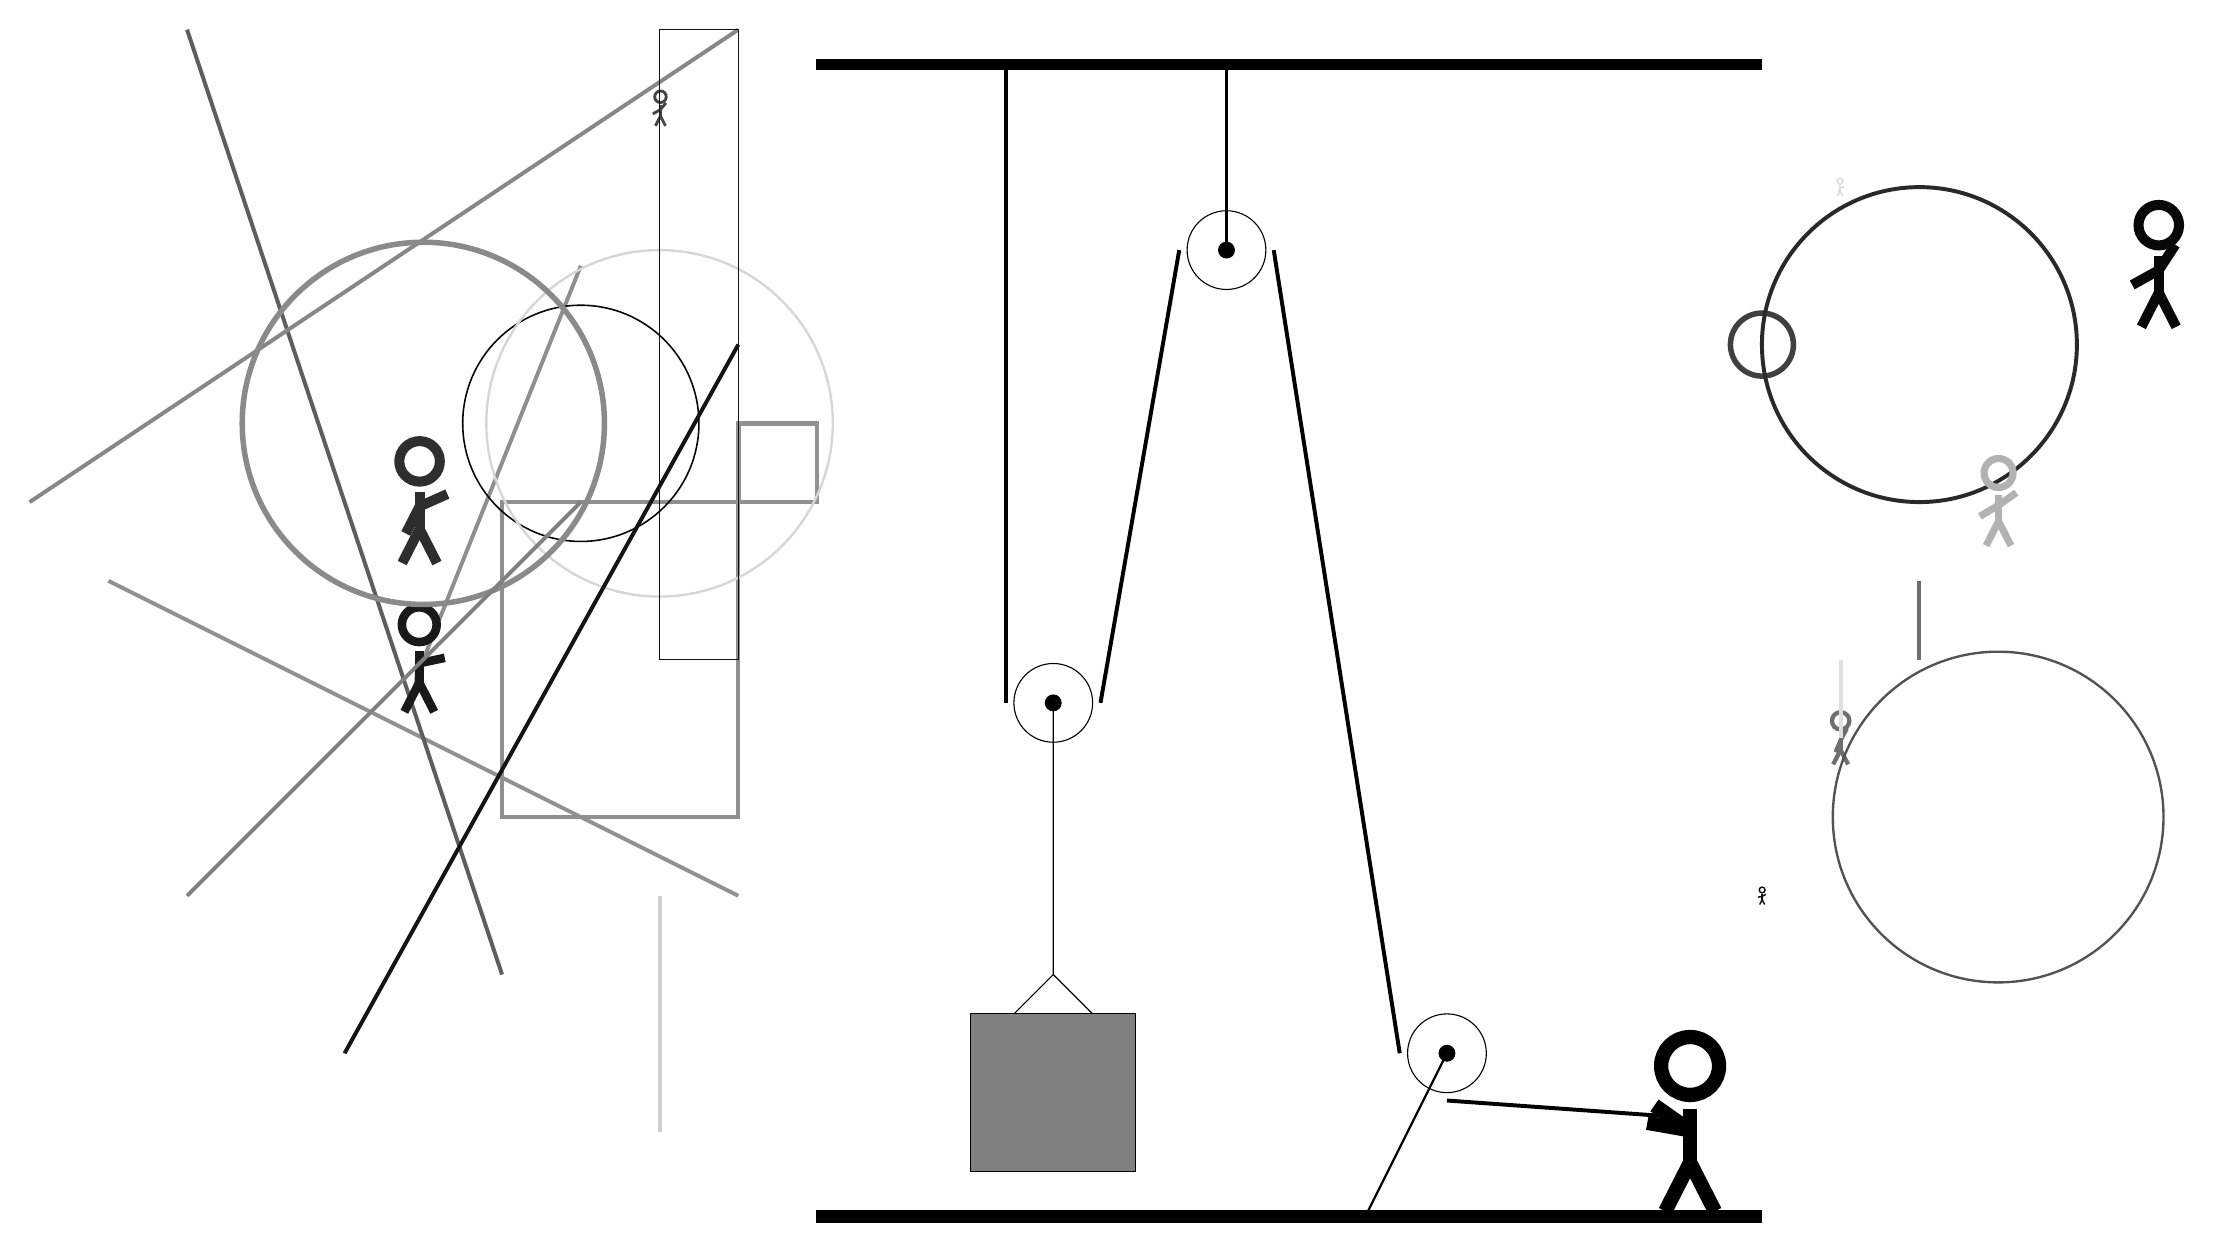
\begin{tikzpicture}
			%%%%% START %%%%%
			
			\draw[fill=black] (-2, 11.5) rectangle (10, 11.625);
			
			\draw[line width=0.5mm, color=black!43](-3, 1) -- (-11, 5);
			
			\draw[line width=0.5mm, color=black!63](-6, 0) -- (-10, 12);
			\draw[line width=0.5mm, color=black!57](12, 4) -- (12, 5);
			\draw[line width=0.5mm, color=black!44](-5, 9) -- (-7, 4);
			\node[line width=0.5mm, color=black!73] at (-4, 11) {\Strichmaxerl[2][29][51]};
			\node[line width=0.2mm, color=black!57] at (11, 3) {\Strichmaxerl[3][67][62]};
			\draw [line width=0.7mm, color=black!75](10, 8) circle (0.4);
			
			\draw[line width=0.5mm, color=black!44] (-3, 6) rectangle (-6, 2);
			\node[line width=0.7mm, color=black!97] at (15, 9) {\Strichmaxerl[7][29][57]};
			
			\node[line width=0.2mm, color=black!90] at (-7, 4) {\Strichmaxerl[6][89][12]};
			
			\draw[line width=0.6mm, color=black!43] (-3, 6) rectangle (-2, 7);
			\draw [line width=0.5mm, color=black!84](12, 8) circle (2.0);
			\node[line width=0.5mm, color=black!82] at (-7, 6) {\Strichmaxerl[7][63][24]};
			\draw[line width=0.5mm, color=black!12](11, 4) -- (11, 3);
			\draw[line width=0.5mm, color=black!47](-3, 12) -- (-12, 6);
			\draw [line width=0.2mm, color=black!98](-5, 7) circle (1.5);
			
			\draw [line width=0.3mm, color=black!16](-4, 7) circle (2.2);
			
			\draw[line width=0.5mm, color=black!92](-3, 8) -- (-8, -1);
			\node[line width=0.2mm, color=black!94] at (10, 1) {\Strichmaxerl[1][10][29]};
			\draw[line width=0.2mm, color=black!93] (-4, 4) rectangle (-3, 12);
			\draw [line width=0.3mm, color=black!68](13, 2) circle (2.1);
			\draw [line width=0.7mm, color=black!46](-7, 7) circle (2.3);
			\node[line width=0.7mm, color=black!30] at (13, 6) {\Strichmaxerl[5][31][35]};
			\node[line width=0.6mm, color=black!14] at (11, 10) {\Strichmaxerl[1][68][15]};
			\draw[line width=0.5mm, color=black!50](-5, 6) -- (-10, 1);
			\draw[line width=0.5mm, color=black!19] (-4, 1) rectangle (-4, -2);
			
			\draw (3.2, 9.2) circle (0.5);
			\draw[fill=black] (3.2, 9.2) circle (0.1);
			\draw[thick] (3.2, 9.2) -- (3.2, 11.5);
			
			\draw (6, -1) circle (0.5);
			\draw[fill=black] (6, -1) circle (0.1);
			\draw[thick] (6, -1) -- (5, -3);
			
			\draw (1, 3.45) circle (0.5);
			\draw[fill=black] (1, 3.45) circle (0.1);
			
			\draw (1, 3.45) -- (1, 0.0) -- (0.5, -0.5);
			\draw (1, 0.0) -- (1.5, -0.5);
			\draw[fill=black!50] (-0.05, -0.5) rectangle (2.05, -2.5);
			
			\draw[line width=0.5mm] (0.4, 11.5) -- (0.4, 3.45);
			\centerarc[line width=0.5mm](1, 3.45)(180:360:0.6);
			\draw[line width=0.5mm](1.6, 3.45) -- (2.6, 9.2);
			\centerarc[line width=0.5mm](3.2, 9.2)(0:180:0.6);
			\draw[line width=0.5mm](3.8, 9.2) -- (5.4, -1);
			\centerarc[line width=0.5mm](6, -1)(180:270:0.6);
			\draw[line width=0.5mm](6, -1.6) -- (8.8, -1.8);
			
			\node at (9, -1.9) {\Strichmaxerl[10][-35][170]};
			
			\draw[fill=black] (-2, -3) rectangle (10, -3.15);
			
			%%%%% END %%%%%
		\end{tikzpicture}
	\end{figure}	
\end{document}